\documentclass[a4paper,hidelinks,14pt]{extarticle}

\usepackage[utf8]{inputenc}
\usepackage[T2A]{fontenc}
\usepackage[english, russian]{babel}
\usepackage{lipsum}
\usepackage{amsmath}
\usepackage{amssymb}
\usepackage{amsfonts}
\usepackage{mathtools}
\usepackage{datetime}
\usepackage[pdftex]{graphicx}
\usepackage{indentfirst}
\usepackage{asymptote}
\usepackage{systeme}
\usepackage[dvipsnames]{xcolor}
\usepackage{lastpage}
\usepackage{fancybox,fancyhdr}
\usepackage{hyperref}
\usepackage[numbered,framed]{matlab-prettifier}
\usepackage[font={small,it}]{caption}
\fancyhead[L]{Лабораторная работа №4}
\fancyhead[C]{}
\fancyhead[R]{Линейная фильтрация}
\fancyfoot[L]{}
\fancyfoot[C]{Страница \thepage\space из \pageref{LastPage}}
\fancyfoot[R]{}
\pagestyle{fancy}
\newcommand{\gt}{\textgreater}
\newcommand{\lt}{\textless}


\begin{document}
	\begin{titlepage}
		\setlength{\parindent}{0ex}
		
		\begin{center}
			\textsc{
				\vspace{1ex}
				Научно исследовательский университет ИТМО \\
				\vspace{0.5ex}
				Факультет систем управления и робототехники \\
				\vspace{0.5ex}
			}
		\end{center}
		
		\vspace{50mm}
		
		\begin{center}
			Отчет по лабораторной работе №4 \\
			Линейная фильтрация
		\end{center}
		
		\vspace{50mm}
		
		\begin{minipage}{.55\linewidth}
			Выполнил студент группы R3280
			
			Преподаватели
		\end{minipage}
		\hfill
		\begin{minipage}{.5\linewidth}
			\begin{flushright}
				Мовчан И. Е.
				\\
				Пашенко А.В., Перегудин А. А.
			\end{flushright}
		\end{minipage}
		
		\vfill
		\begin{center}
			Санкт-Петербург
			\\
			2024
		\end{center}
		
	\end{titlepage}
	
	\section{Спектральное дифференцирование}
	
	Воспользуемся следующим кодом:

	\begin{lstlisting}[style=Matlab-editor, basicstyle=\footnotesize, caption={Базовый код}]
a = 0.5;
dt = 0.25;
t = -100:dt:100;
y = sin(t);
y = y + a*(rand(size(t))-0.5);lstconsolas

g = zeros(1,length(t));
for k = 1:(length(t)-1)
	g(k) = (y(k+1) - y(k))/dt;
end
g(length(t)) = 0;

vx = -1:dt:1;
furie = zeros(1, length(vx));
for k = 1:length(vx)
	furie(k) = 2*pi*1i*vx(k)*trapz(t, y.*exp(-2*pi*1i*vx(k)*t));
end

der = zeros(1,length(t));
for k = 1:length(t)
	der(k) = trapz(vx, furie.*exp(2*pi*1i*vx*t(k)));
end		
	\end{lstlisting}
	
	Здесь мы задаёмся массивом времени $t$, зашумлённым сигналом $y$, после чего численно находим спектральную производную пользуясь тем фактом, что Фурье-образ производной сигнала связан с Фурье-образом домножением на $2\pi i \nu $.
	
	Графики спектральной и численной производных вместе и истинной производной $\cos(t)$ сигнала представлены на рисунке \ref{1}.
	\begin{figure}[h]
		\centering
		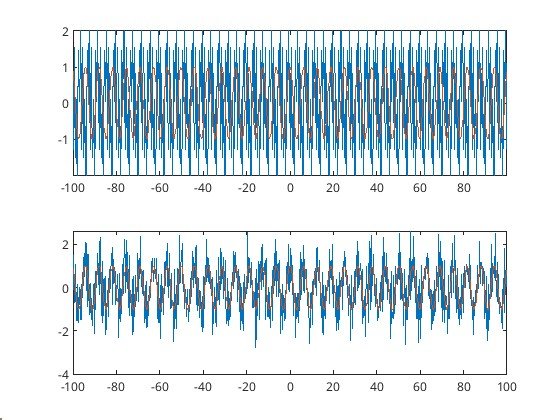
\includegraphics[scale=0.75]{./images/1.jpg}
		\caption{Графики спектральной и численной производных}
		\label{1}
	\end{figure}
	
	
\end{document}